\documentclass[class=minimal,border=0pt]{standalone}

\usepackage{xcolor}
\usepackage{amsmath, amsfonts, mathtools, amssymb, amsthm} 
\usepackage{tikz, pgfplots}
\usetikzlibrary{chains, shapes,arrows,automata,decorations,trees, backgrounds, patterns, calc, matrix}
\pgfplotsset{compat=1.8}
\DeclareMathOperator{\parab}{par}
\definecolor{darkgreen}{rgb}{0.0 0.5 0.0}
\definecolor{whitegreen}{rgb}{0.0 0.75 0.0}
\definecolor{whiteblue}{rgb}{0.0 0.0 1.2}
\definecolor{darkred}{rgb}{0.8 0.0 0.0}
\def\samplepar{10}
\def\sampleatn{30}
\def\samplesamp{35}
\newcommand{\xc}{\mathbf{x}_c^*}
\newcommand{\Ballr}[1]{\mathcal{B}_{#1, r}}
\usepackage{listings}
\def\lstlanguagefiles{defManOcaml.tex}
\lstset{language = Ocaml}
\newcommand{\fpop}{f_{\text{pop}}}
\newcommand{\Add}[2]{\mathtt{Add} \ (#1) (#2)}
\newcommand{\Mult}[2]{\mathtt{Mult} \ (#1) (#2)}
\newcommand{\Ineq}[1]{\mathtt{Ineq} \ #1}
\newcommand{\Sos}[1]{\mathtt{Sos} \ #1}
\newcommand{\Obj}[1]{\mathtt{Obj} \ #1}
%nodes = {node/.style = {circle,minimum size=\myunit}},
%nodes = {align=center, text width = 2cm},
\begin{document} 
\newcommand{\myunit}{1 cm}

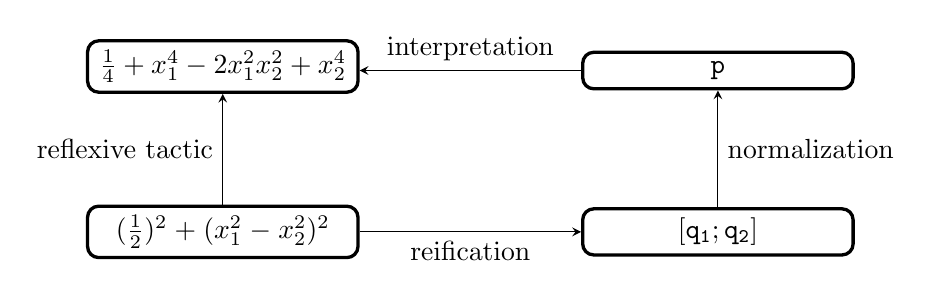
\begin{tikzpicture}
\tikzset{
    node style sp/.style={draw,rectangle,minimum size=\myunit}
    %node style ge/.style={circle,minimum size=\myunit},
    %arrow style mul/.style={draw,sloped,midway,fill=white},
    %arrow style plus/.style={midway,sloped,fill=white},
}
  \matrix (m) [matrix of nodes, nodes = {style={draw,rectangle, rounded corners, draw=black, very thick}, align=center, text width = 3.2cm}, row sep=4em, column sep=8em]
  {
     $\frac{1}{4} + x_1^4 - 2 x_1^2 x_2^2 + x_2^4$       & $\mathtt{p}$ \\
     $(\frac{1}{2})^2 + (x_1^2 - x_2^2)^2$ & {$\mathtt{[q_1; q_2]}  $ }\\};
  \path[-stealth]
    (m-2-1) edge node [left] {reflexive tactic} (m-1-1)
            %edge [double] node [above] {reification} (m-1-2)
    (m-2-1) edge node [below] {reification} (m-2-1-|m-2-2.west)
    (m-1-2) edge node [above] {interpretation} (m-1-2-|m-1-1.east)
%            node [above] {reification} 
            
    (m-2-2) edge node [right] {normalization} (m-1-2);
           % edge [dashed,-] (m-2-1);
\end{tikzpicture}

 \end{document}